\begin{figure}
    \centering
    \newcommand*{\subfigwidth}{0.49\textwidth}
    \begin{subfigure}[b]{\subfigwidth}
        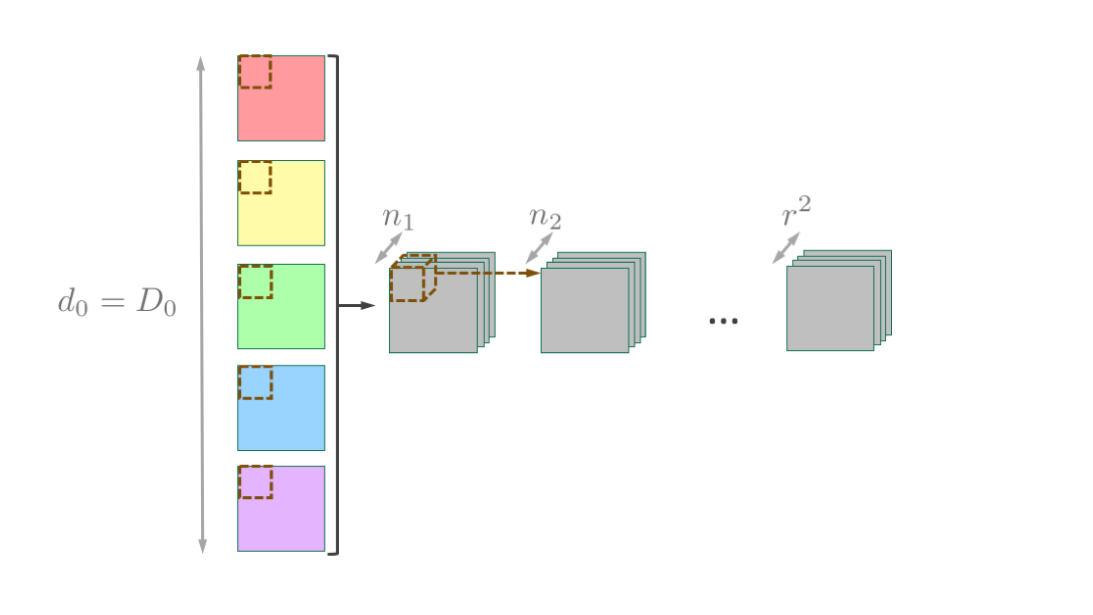
\includegraphics[width=\linewidth,keepaspectratio]{figures/neural_networks/early_fusion.png}
        \caption{Early fusion.}\label{subfig:earlyfus}
    \end{subfigure}
    \vskip\baselineskip
    \begin{subfigure}[b]{\subfigwidth}
        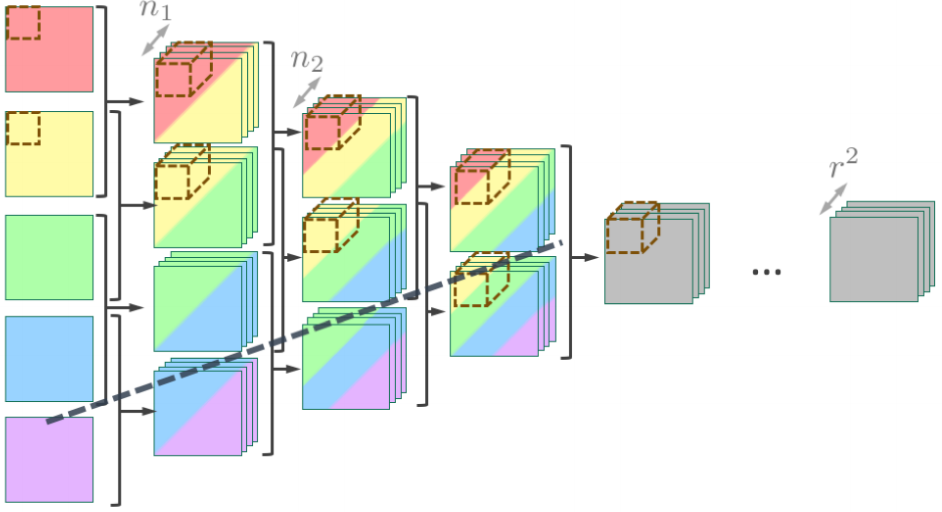
\includegraphics[width=\linewidth,keepaspectratio]{figures/neural_networks/slow_fusion.png}
        \caption{Slow fusion.}\label{subfig:updowndbpn}
    \end{subfigure}
    \vskip\baselineskip
    \begin{subfigure}[b]{\subfigwidth}
        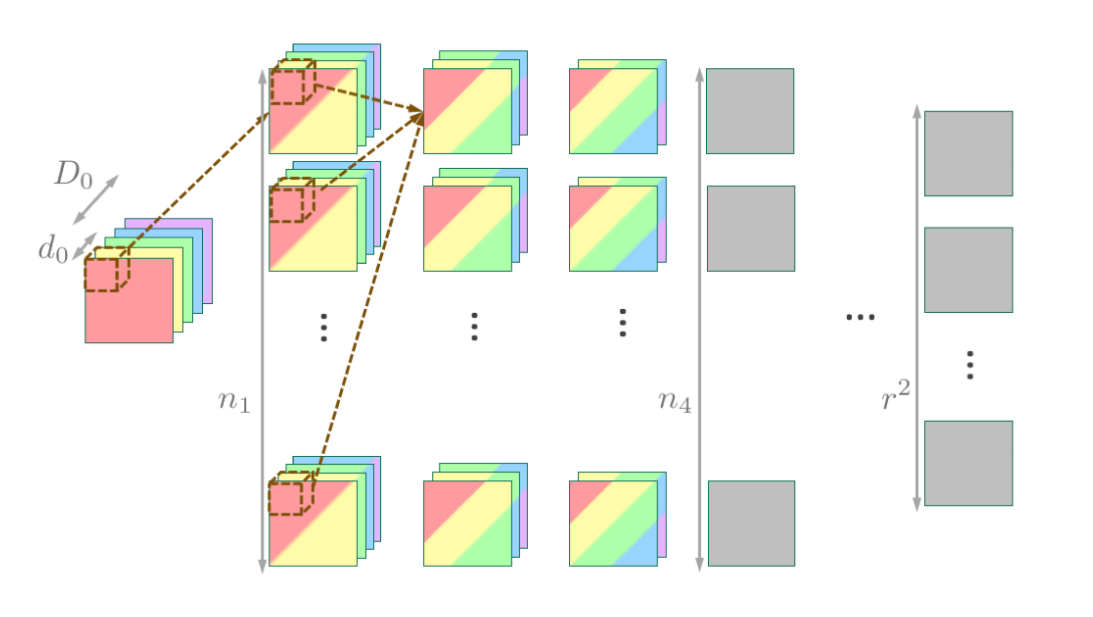
\includegraphics[width=\linewidth,keepaspectratio]{figures/neural_networks/3d_conv.png}
        \caption{3D convolution.}\label{subfig:updowndbpn}
    \end{subfigure}
    \caption{Space-time models\cite{caballero2017real}}\label{fig:fusions}
\end{figure}